\chapter{บทนำ}
\section{ที่มาและความสำคัญ}

\hspace{1cm} ในปัจจุบันการใช้ภาพดิจิตัล (digital images) ในสังคมเครือข่ายได้รับความนิยมอย่างแพร่หลาย เนื่องจากโทรศัพท์เคลื่อนที่มีราคาถูกลงแต่มีความสามารถที่ชาญฉลาด สามารถทำหน้าที่ได้ตั้งแต่การเป็นกล้องดิจิตัลคอมแพค (compact digital camera)  คุณภาพดีให้ภาพดิจิตัลที่มีความคมชัดสูงจนไปถึงการทำหน้าที่ดังเช่นเครื่องคอมพิวเตอร์ส่วนบุคคลที่สามารถเชื่อมต่อกับระบบเครือข่ายไร้สายเพื่อรับส่งภาพดิจิตัลในสังคมเครือข่ายด้วยความสะดวกและรวดเร็ว

\hspace{1cm} นอกจากภาพดิจิตัลจะได้รับจากการถ่ายภาพด้วยโทรศัพท์เคลื่อนที่แล้ว ภาพดิจิตัลยังได้รับการถ่ายภาพด้วยกล้องดีเอสแอลอาร์ หรือ กล้องสะท้อนเลนส์เดี่ยวแบบดิจิตัล (digital single lens reflex camera) กล้องโทรทรรศน์ (หรือ กล้องดูดาว) หรือ เครื่องมือสร้างภาพถ่ายทางการแพทย์ (medical imaging device) 

\hspace{1cm} โดยทั่วไปภาพดิจิตัลจะได้รับการประมวลผลภาพก่อนนำไปใช้งานเพื่อให้สามารถใช้ข้อมูลที่ปรากฎบนภาพได้ตรงวัตถุประสงค์ของการใช้งานมากที่สุด ตัวอย่างเช่น ภาพบุคคล (portrait) อาจจำเป็นต้องได้รับการกำจัดสัญญาณรบกวนออกจากภาพและ/หรือปรับเพิ่มความละเอียดข้อมูลของความเข้มของสีและความสว่างของสีบนบริเวณใบหน้าก่อนนำภาพไปใช้งานเพื่อจัดทำต้นฉบับวารสารหรือหนังสือของสำนักพิมพ์ เป็นต้น  

\hspace{1cm} การต่อเติมภาพ (image inpainting) เป็นวิธีการประมวลผลภาพชนิดหนึ่งมีเป้าหมายเพื่อซ่อมแซมภาพด้วยการต่อเติมข้อมูลของความเข้มของสีบนบริเวณที่กำหนด (ต่อไปจะเรียกบริเวณนี้ว่าโดเมนต่อเติม (inpainting domain)) โดยอาศัยข้อมูลของความเข้มของสีที่ปรากฏในภาพ ตัวอย่างเช่น 
กำหนดให้รูปที่ \ref{figure:inpaint-explain} (\subref{figure:inpaint-explain:to-inpaint}) แสดงภาพที่ต้องการซ่อมแซมระดับความเข้มของสีบนบริเวณแท่งวัตถุรูปร่างสี่เหลี่ยมสีขาว การต่อเติมภาพดังกล่าวจะเริ่มด้วยการกำหนดให้บริเวณแท่งวัตถุรูปร่างสี่เหลี่ยมสีขาวเป็นโดเมนการต่อเติมดังรูปที่ \ref{figure:inpaint-explain} (\subref{figure:inpaint-explain:inpaint-domain})  จากนั้นภาพที่ได้รับการซ่อมแซมหรือภาพที่ได้รับการต่อเติม (restored or inpainted image) ซึ่งแสดงในรูปที่ \ref{figure:inpaint-explain} (\subref{figure:inpaint-explain:inpainted}) ได้มาจากขั้นตอนวิธีการต่อเติมภาพ (inpainting algorithm) ซึ่งได้รับการออกแบบเพื่อนำข้อมูลที่ปรากฎบนภาพในบริเวณใกล้เคียงกับขอบของโดเมนต่อเติมมาซ่อมแซมภาพ 
	
\begin{figure}[H]
	\centering
	\begin{subfigure}{0.3\linewidth}
		\centering
		
\includegraphics[width=0.8\linewidth]{image/grayscale_inpaint/toinpaint.png}
        \caption{ภาพที่ต้องการซ่อมแซม}
        \label{figure:inpaint-explain:to-inpaint}
	\end{subfigure}
	\begin{subfigure}{0.3\linewidth}
		\centering
		
\includegraphics[width=0.8\linewidth]{image/grayscale_inpaint/inpaintdomain.png}
        \caption{โดเมนต่อเติม}
        \label{figure:inpaint-explain:inpaint-domain}
	\end{subfigure}
	\begin{subfigure}{0.3\linewidth}
		\centering
		
\includegraphics[width=0.8\linewidth]{image/grayscale_inpaint/result_splitbergman.png}
        \caption{ภาพที่ได้รับการซ่อมแซม}
        \label{figure:inpaint-explain:inpainted}
	\end{subfigure}
	\caption{ตัวอย่างการซ่อมแซมภาพ}
	\label{figure:inpaint-explain}
\end{figure}

\hspace{1cm} เท่าที่ผู้วิจัยศึกษาและค้นคว้ามาจนถึงขณะนี้ ผู้วิจัยพบว่าการต่อเติมภาพมักนิยมนำไปใช้งานสำหรับการปรับแต่งความสวยงามของภาพบุคคลที่ถ่ายจากโทรศัพท์เคลื่อนที่ เช่น การลบร่องรอยของรอยตีนกา การลบร่องรอยแผลเป็นที่เกิดจากสิวเสี้ยน การลดร่องรอยของความชรา หรือ การเพิ่มความใสและความเนียนของสีผิวบนบริเวณใบหน้าผ่านโปรแกรมแอปพลิเคชันแต่งรูปภาพที่มีอยู่ในแอปสโตร์ (App Store) หรือ กูเกิ้ลเพลย์ (Google Play) เป็นต้น 
	
\subsection{การซ่อมแซมภาพจิตรกรรมไทยโบราณ}

\hspace{1cm} ภาพจิตรกรรมไทย คือ ภาพเขียนที่มีเอกลักษณ์ความเป็นศิลปะไทยซึ่งโดดเด่นและแตกต่างจากภาพเขียนของชนชาติอื่น ในอดีต  ช่างไทยได้สร้างสรรค์ลวดลายและสีสันบนภาพวาดเพื่อสะท้อนประเพณีและวัฒนธรรมในสังคมไทยที่เกี่ยวกับศาสนา ประวัติศาสตร์ โบราณคดี ชีวิตความเป็นอยู่ วัฒนธรรมการแต่งกาย ตลอดจนการแสดงการเล่นพื้นเมืองต่าง ๆ ของแต่ละยุคสมัย 
	
\hspace{1cm} อย่างไรก็ตาม ภาพจิตรกรรมไทยจำนวนไม่น้อยที่เสื่อมสลายตามกาลเวลา และรอคอยการซ่อมแซมจากช่างในสมัยปัจจุบันที่ต้องไม่สร้างความเสียหายให้กับภาพเขียนเพิ่มขึ้นมากกว่าเดิม  ที่ผ่านมาภาพที่ผ่านการซ่อมแซมมาแล้วจำนวนไม่น้อยได้รับความเสียหายหลังจากการซ่อมแซม ถึงแม้สภาพโดยรวมของภาพจิตรกรรมเดิมยังคงอยู่ แต่รายละเอียดในตัวภาพเขียนได้เปลี่ยนไป ก่อให้เกิดความเสียหายที่ประเมินค่าไม่ได้ 
	
\hspace{1cm} การซ่อมแซมภาพจิตรกรรมไทยโบราณโดยใช้การต่อเติมภาพเป็นขั้นตอนของการซ่อมแซมแบบหนึ่งซึ่งไม่ก่อให้เกิดความเสียหายใด ๆ กับภาพเดิม เนื่องจากเป็นการซ่อมแซมโดยการใช้ขั้นตอนวิธีเชิงตัวเลขบนภาพดิจิตัลซึ่งเป็นสำเนาของภาพเดิม ด้วยเหตุผลดังกล่าว ผู้วิจัยได้เล็งเห็นว่าการซ่อมแซมภาพจิตรกรรมไทยโบราณมีความจำเป็นเร่งด่วน เนื่องจากภาพที่ได้รับการซ่อมแซมด้วยการต่อเติมภาพสามารถนำไปใช้ประกอบการตัดสินใจเพื่อวางแผนก่อนการลงมือซ่อมแซมภาพเขียนจริงได้ นอกจากนี้ ขั้นตอนวิธีการต่อเติมภาพสามารถนำไปใช้สร้างแอปพลิเคชันบนโทรศัพท์เคลื่อนที่เพื่อในไปใช้เป็นข้อมูลในการเข้าชมภาพเขียนเดิมที่ยังไม่ได้รับการซ่อมแซมและภาพเขียนที่ได้รับการซ่อมแซมโดยวิธีการทางคณิตศาสตร์จากแอปพลิเคชันที่พัฒนาขึ้น
	
\hspace{1cm} รูปที่ \ref{figure:inpaint-thaiairt-explain} แสดงตัวอย่างภาพจิตรกรรมไทย\footnote{ภาพถ่ายที่วัดภูมินทร์ อำเภอเมือง จังหวัดน่าน; ภาพจาก http://topicstock.pantip.com/camera/topicstock/2009/02/O7514399/O7514399.html สืบค้นเมื่อวันที่ 23 กันยายน 2561} ที่ต้องได้รับการซ่อมแซมบนบริเวณแขนเสื้อของรูปวาดผู้ชายที่มีส่วนของสีแดงเดิมหลุดหายไป ทั้งนี้ในการซ่อมแซมภาพโดยการต่อเติมภาพ เราจะเริ่มด้วยการสร้างโดเมนต่อเติมบนบริเวณสีพื้นผิวปูนที่แขนเสื้อ จากนั้นจึงนำขั้นตอนวิธีการต่อเติมภาพเพื่อซ่อมแซมภาพบริเวณนั้นให้เป็นสีแดง 

\begin{figure}[h]
	\[
	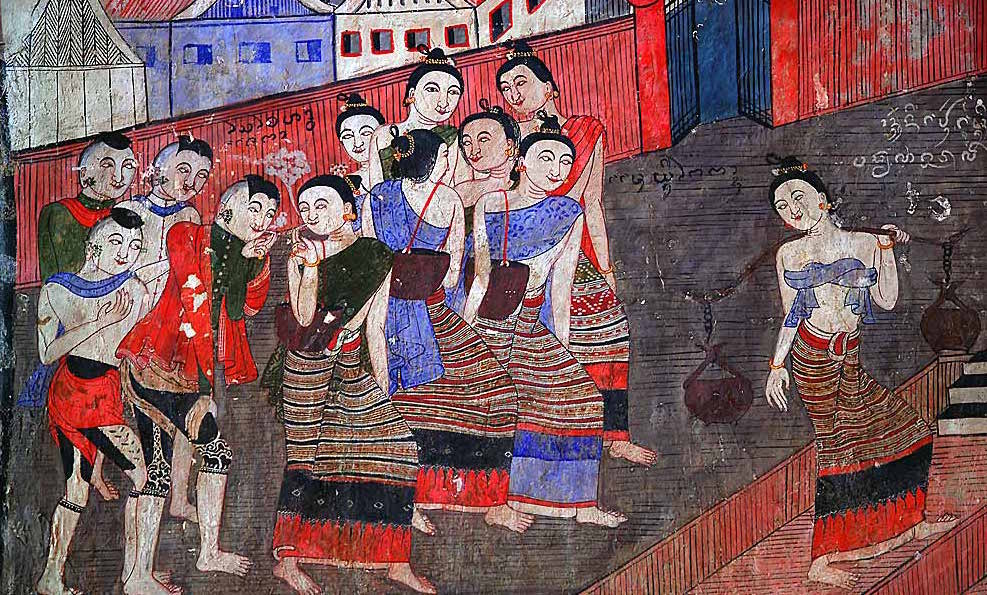
\includegraphics[width=0.6\linewidth]{image/explain_art/fig2a.jpg}
	\]
	\caption{ภาพจิตรกรรมไทยที่วัดภูมินทร์ อำเภอเมือง จังหวัดน่าน}
	\label{figure:inpaint-thaiairt-explain}
\end{figure}

\subsection{การลบบทบรรยายบนอนิเมะ}
\hspace{1cm}อนิเมะคือวิดีโอภาพวาดการ์ตูนสไตล์ญี่ปุ่นซึ่งเป็นที่นิยมของเยาวชนไทย ในการรับชมอนิเมะ แม้ว่าเยาวชนไทยสามารถรับชมด้วยบทพากย์เสียงภาษาไทย แต่ก็สูญเสียอรรถรสของการรับชมจากบทบรรยายแบบแข็ง\footnote{บทยรรยายที่ไม่สามารถปิดหรือเปิดได้} (hardsub) ที่เป็นภาษาต่างประเทศในบริเวณด้านล่างของจอภาพ ในการซ่อมแซม\\อนิเมะด้วยการลบบทบรรยายภาษาต่างประเทศจึงเป็นงานที่ยุ่งยากและท้าท้ายมาก เนื่องจาก
\begin{itemize}
	\item [(1)] อนิเมะเป็นวิดีโอซึ่งแสดงผลประมาณ 24 เฟรม(ภาพ)ต่อวินาที
	\item [(2)] แต่ละเฟรมอาจมีหรืออาจไม่มีบทบรรยายก็ได้
	\item [(3)] แต่ละเฟรมอาจมีหรืออาจไม่มีบทบรรยายเดียวกันก็ได้
	\item [(4)] แต่ละเฟรมเป็นการแสดงผลภาพสีที่มีระดับความคมชัดสูง (high definition) ขนาดมากถึง $1920\times1080$ พิกเซล
\end{itemize}
ด้วยความท้าทายข้างต้น การพัฒนาขั้นตอนวิธีการต่อเติมภาพที่สามารถกำหนดโดเมนต่อเติมเชิงอัตโนมัติให้กับแต่ละเฟรมและประมวลผลได้แม่นยำจนการลบบทบรรยายสามารถทำงานได้แบบเรียลไทม์จึงเป็นสิ่งจำเป็นที่หลีกเลี่ยงไม่ได้
	
\hspace{1cm} รูปที่ \ref{figure:inpaint-anime-explain} แสดงตัวอย่าง 1 เฟรมของอนิเมะที่มีบทบรรยายแบบแข็ง\footnote{ภาพจาก https://www.samehadaku.tv/2018/07/grand-blue-episode-1-subtitle-indonesia.html สืบค้นเมื่อวันที่ 23 กันยายน 2561} ที่ต้องซ่อมแซมด้วยการลบบทบรรยายออก  ทั้งนี้ในการลบบทบรรยายออกจากเฟรมโดยใช้การต่อเติมภาพ เราจะเริ่มด้วยการสร้างโดเมนต่อเติมแบบอัตโนมัติในบริเวณบทบรรยาย จากนั้นจึงนำขั้นตอนวิธีการต่อเติมภาพแบบเร็วเพื่อลบบทบรรยายออกจากเฟรม 

\begin{figure}[h]
    \[
    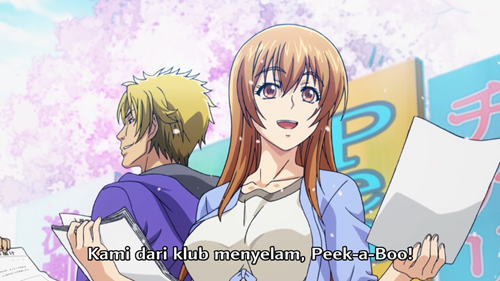
\includegraphics[width=0.42\linewidth]{image/explain_art/fig3.png}
    \]
    \caption{1 เฟรมของอนิเมะที่มีบทบรรยายแบบแข็ง}
    \label{figure:inpaint-anime-explain}
\end{figure}
	
\hspace{1cm} โครงการวิจัยนี้ ผู้วิจัยมีเป้าหมายสำคัญคือการพัฒนาขั้นตอนวิธีการต่อเติมภาพแบบเร็วและแม่นยำชนิดใหม่เพื่อนำไปใช้สำหรับซ่อมแซมภาพจิตรกรรมไทยและการลบบทบรรยายออกจากอนิเมะ

\clearpage
	